\documentclass{article}
\usepackage{amsmath}
\usepackage[mathletters]{ucs}
\usepackage[utf8x]{inputenc}
\usepackage[margin=1.5in]{geometry}
\usepackage{enumerate}
\newtheorem{theorem}{Theorem}
\usepackage[dvipsnames]{xcolor}
\usepackage{pgfplots}
\pgfplotsset{compat=1.18}
\setlength{\parindent}{0cm}
\usepackage{graphics}
\usepackage{graphicx} % Required for including images
\usepackage{subcaption}
\usepackage{bigintcalc}
\usepackage{pythonhighlight} %for pythonkode \begin{python}   \end{python}
\usepackage{appendix}
\usepackage{arydshln}
\usepackage{physics}
\usepackage{tikz-cd}
\usepackage{booktabs} 
\usepackage{adjustbox}
\usepackage{mdframed}
\usepackage{relsize}
\usepackage{physics}
\usepackage[thinc]{esdiff}
\usepackage{fixltx2e}
\usepackage{esint}  %for lukket-linje-integral
\usepackage{xfrac} %for sfrac
\usepackage{hyperref} %for linker, må ha med hypersetup
\usepackage[noabbrev, nameinlink]{cleveref} % to be loaded after hyperref
\usepackage{amssymb} %\mathbb{R} for reelle tall, \mathcal{B} for "matte"-font
\usepackage{listings} %for kode/lstlisting
\usepackage{verbatim}
\usepackage{graphicx,wrapfig,lipsum,caption} %for wrapping av bilder
\usepackage{mathtools} %for \abs{x}
\usepackage[norsk]{babel}
\definecolor{codegreen}{rgb}{0,0.6,0}
\definecolor{codegray}{rgb}{0.5,0.5,0.5}
\definecolor{codepurple}{rgb}{0.58,0,0.82}
\definecolor{backcolour}{rgb}{0.95,0.95,0.92}
\lstdefinestyle{mystyle}{
    backgroundcolor=\color{backcolour},   
    commentstyle=\color{codegreen},
    keywordstyle=\color{magenta},
    numberstyle=\tiny\color{codegray},
    stringstyle=\color{codepurple},
    basicstyle=\ttfamily\footnotesize,
    breakatwhitespace=false,         
    breaklines=true,                 
    captionpos=b,                    
    keepspaces=true,                 
    numbers=left,                    
    numbersep=5pt,                  
    showspaces=false,                
    showstringspaces=false,
    showtabs=false,                  
    tabsize=2
}

\lstset{style=mystyle}
\author{Oskar Idland}
\title{Oblig 6}
\date{}
\begin{document}
\maketitle
\newpage

\section*{\underline{A Diskusjonsoppgaver}}
\subsection*{Oppgave 1}
\subsubsection*{a)}
\paragraph*{Definisjon}
Ortonormalitet er definert som at indreproduktet mellom to egenfunksjoner er null hvis de er ulike og ett hvis de er like, notert ned Kronecker delta. For funksjoner defineres det i et område. Dette kan være i et vilkårlig intervall $[a,b]$, som inkluderer $[-∞, ∞]$ . Det vil si at 
\[
\braket{ψ_i}{ψ_j} = ∫_{-∞}^{∞} ψ_i^{*} ψ_j = δ_{ij} = \begin{cases} 
1 & \text{hvis } i = j \\ 
0 & \text{hvis } i ≠ j 
\end{cases}
\]
For egentilstandene til en partikkel betyr dette hvis en partikkel måles i en tilstand $ψ_i$ vil den ikke kunne måles i en tilstand $ψ_j$ rett etterpå. 
\subsubsection*{b)}
Bølgefunksjonen må være normalisert ettersom $∫_{-∞}^{∞} Ψ^{*}Ψ \ \mathrm{d}$ må være lik 1. Det er fordi utrykket representer sannsynligheten for å finne en partikkel en plass i universet, som selvfølgelig må være 1.
\subsubsection*{c)}
Ja, ettersom integralet er med hensyn til $x$ har det ikke noe å si om vi legger til en faktor gitt av $t$. 

\subsection*{Oppgave 2}
\subsection*{a)}
Svaret er \underline{nei, aldri}, ettersom ved måling vil $Ψ$ kollapse til en av sine egentilstander, og sin tilhørende energi. I vårt tilfelle er det $E_1$ eller $E_2$. 

\subsubsection*{b)}
Resultatet av en energimåling av $Ψ_{\text{sum}}$ vil kollapse Bølgefunksjonen til enten $Ψ_1$ eller $Ψ_2$ som vil gi oss en energi som er enten $E_1$ eller $E_2$.

\subsubsection*{c)}
Forventningsverdien $\left<E\right>$ vil ikke være det samme som målingen i oppgave b), ettersom $\left<E\right>$ representerer et gjennomsnitt fra flere målinger, ikke bare energien fra én måling, slik at $\left<E\right> ∈ \left<E_1, E_2\right> $

\subsubsection*{d)}
Den nye bølgefunksjonen vil se ut som enten $Ψ_1$ eller $Ψ_2$ avhengig av hva målingen av $Ψ_{\text{sum}}$ kollapser til. Da vil vi også måle energien tilhørende til den respektive bølgefunksjonen, enten $E_1$ eller $E_2$. 
  
\subsubsection*{e)}
Hvis systemet er beskrevet av $Ψ_1$ alene vil vi alltid måle den tilhørende energien $E_1$. 

\subsection*{Oppgave 3}
\underline{B: Det er en energi-tilstand, og den er proporsjonal med tilstanden $ψ_n$}. 
Dette er logisk ettersom $\hat{a}_{+}ψ_n = ψ_{n+1} /\sqrt{n!} $

\section*{\underline{B Regneoppgaver}}
\subsection*{Oppgave 4}
\subsubsection*{a)}
Grunntilstanden er gitt ved 
\begin{equation}
ψ_0 = \left(\frac{mω}{πℏ}\right)^{\frac{1}{4}} e^{-\frac{mω}{2ℏ}x^2} \label{eq:psi0}
\end{equation}
Heveoperatoren som beskrevet i Griffiths likning 2.48 (versjon 3) gjør følgende
\begin{equation}\label{eq: a_+}
\hat{a}_{+} = \frac{1}{\sqrt{2ℏmω}} \left(- i\hat{p} + mωx\right), \quad \hat{p} = -iℏ \frac{\mathrm{d}}{\mathrm{d}x}
\end{equation}
\begin{align*}
ψ_1 &= \hat{a}_{+} ψ_0 
\\
ψ_1 &= \frac{1}{\sqrt{2ℏmω}} \left(\frac{mω}{πℏ}\right)^{\frac{1}{4}} \left(-i\hat{p}e^{-\frac{mω}{2ℏ}x^2} + mωx e^{-\frac{mω}{2ℏ}x^2}\right) 
\\
ψ_1 &=\frac{1}{\sqrt{2ℏmω}}\left(\frac{mω}{πℏ}\right)^{\frac{1}{4}} \left(mωx + mωx\right) e^{-\frac{mω}{2ℏ}x^2} \\ 
ψ_1 &= \frac{2mωx}{\sqrt{2ℏmω}}\left(\frac{mω}{πℏ}\right)^{\frac{1}{4}} e^{-\frac{mω}{2ℏ}x^2} 
\\
ψ_1 &= \underline{\underline{\sqrt{\frac{2mω}{ℏ}}x ψ_0}}
\end{align*}
Videre har vi at $ψ_2 = \hat{a}_{+}ψ_1 / \sqrt{2}$. 
\begin{align*}
ψ_2 &= \frac{\hat{a}_{+} ψ_1}{\sqrt{2}}
\\
ψ_2 &= \frac{1}{\sqrt{2}} \frac{1}{2ℏmω} \left(\frac{mω}{πℏ}\right)^{\frac{1}{4}}\left(-ℏ \frac{\mathrm{d}}{\mathrm{d}x}2mωx e^{-\frac{mω}{2ℏ}x^2} + (mωx)^2 e^{- \frac{mω}{2ℏ}x^2}\right)
\\
ψ_2 &= \frac{1}{\sqrt{2}} \frac{1}{2ℏmω} \left(\frac{mω}{πℏ}\right)^{\frac{1}{4}} \left(-2ℏmωe^{-\frac{mω}{2ℏ}x^2} + 2(mωx)^2 e^{- \frac{mω}{2ℏ}x^2} + (mωx)^2 e^{- \frac{mω}{2ℏ}x^2}\right)
\\
ψ_2 &= \frac{1}{\sqrt{2}} \frac{1}{2ℏmω} \left(\frac{mω}{πℏ}\right)^{\frac{1}{4}}\left(-2ℏmω + 3(mωx)^2\right)e^{- \frac{mω}{2ℏ}x^2}
\\
ψ_2 &= \underline{\underline{\frac{1}{\sqrt{2}} \left( \frac{3mω}{2ℏ}x^2 - 1\right)ψ_0}}
\end{align*}

\subsubsection*{b)}
Vi bruker utrykket for potensialet $V(x)$ som beskrevet i Griffiths likning 2.43 (versjon 3)
\begin{equation}\label{eq: V(x)}
V(x) = \frac{1}{2}kx^2
\end{equation}
\begin{figure}[h!]
  \centering
  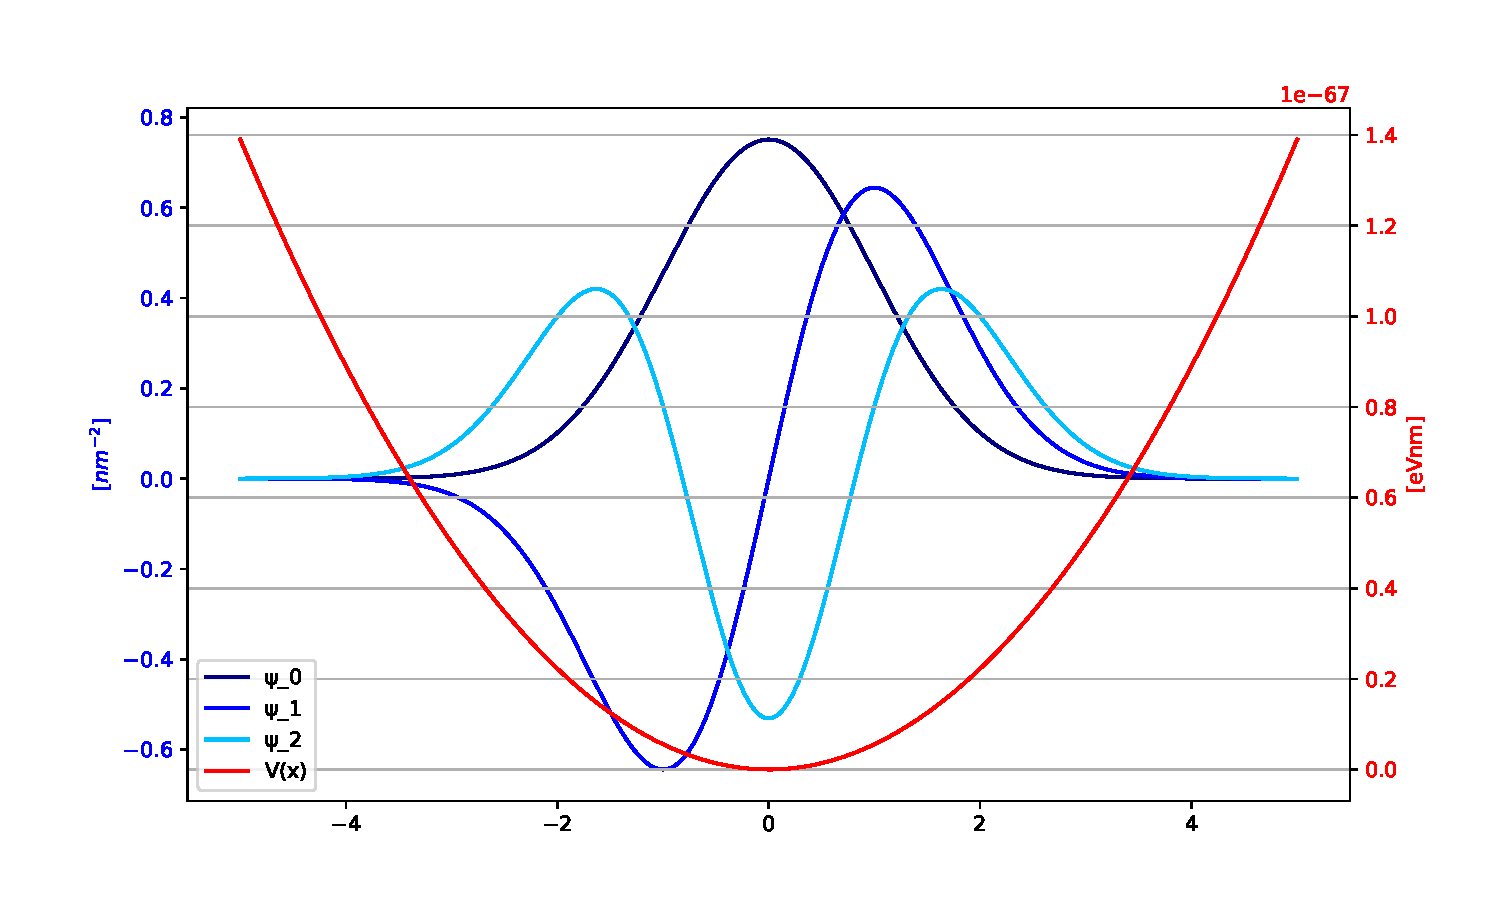
\includegraphics[width = \textwidth]{4b.pdf}
  \caption{Plot av $ψ_0, ψ_1, ψ_2$ og potensialet $V$}
  \label{fig: 4.b}
\end{figure}


\subsubsection*{c)}
Vi sjekker først ortogonaliteten til $ψ_0$ og $ψ_1$. 
\begin{align*}
∫_{-∞}^{∞} ψ_0 ψ_1 \ \mathrm{d}x = ∫_{-∞}^{∞} \sqrt{\frac{2mω}{ℏ}}x ψ_0^2 \ \mathrm{d}x
\end{align*}
Ettersom $ψ_0$ er en parfunksjon symmetrisk om $x=0$ og $x$ er en oddefunksjon symmetrisk om $x=0$ vet vi at et integral symmetrisk om $x=0$ vil være 0. \newline

Videre sjekker vi ortogonaliteten til $ψ_0$ og $ψ_2$. Vi starter med å sette $k = mω / πℏ$

\begin{align*}
  ∫_{-∞}^{∞} ψ_0ψ_2 \ \mathrm{d}x = ∫_{-∞}^{∞} \frac{1}{\sqrt{2}}\left(\frac{3}{2}kx^2 - 1\right)ψ_0^2 \ \mathrm{d}x \\
  \\
  \frac{1}{\sqrt{2}}\left(\underbrace{∫_{-∞}^{∞} \frac{3}{2}kx^2 ψ_0^2 \ \mathrm{d}x }_{\text{utrykk 1}}- \underbrace{∫_{-∞}^{∞} ψ_0^2 \ \mathrm{d}x} _{\text{utrykk 2}} \right) = 0
\end{align*} 



Til slutt sjekker vi ortogonaliteten til $ψ_1$ og $ψ_2$
\begin{align*}
∫_{-∞}^{∞} ψ_1ψ_2 \ \mathrm{d}x = ∫_{-∞}^{∞} \left(\sqrt{2k}xψ_0\right) \left(\frac{1}{\sqrt{2}} \left(\frac{3}{2}kx^2 - 1\right)ψ_0\right) \ \mathrm{d}x
\\
\underbrace{∫_{-∞}^{∞} \frac{3}{2}  \sqrt{k}x^3ψ_0^2 \ \mathrm{d}x}_{\text{= 0 pga symmetri}} - \underbrace{∫_{-∞}^{∞} \sqrt{2k}xψ_0^2 \ \mathrm{d}x}_{\text{= 0 pga symmetri}}
\end{align*}
\subsection*{Oppgave 5}
\subsubsection*{a)}
Vi setter $x = \frac{ξ}{\sqrt{π}α^2}$ og $\mathrm{d}x = \frac{1}{\sqrt{π}α^2} \ \mathrm{d}ξ$
\begin{enumerate}[\bf I]
\item 
\begin{align*}
\left<x\right> &= ∫_{-∞}^{∞} ψ_0^{*}xψ_0 \ \mathrm{d}x 
\\
    &= ∫_{-∞}^{∞} α^2e^{-ξ^2}x \ \mathrm{d}x
\\ 
    &= ∫_{-∞}^{∞} α^2e^{-ξ^2} \frac{ξ}{πα^4} \ \mathrm{d}ξ
\\
    &= \frac{1}{πα^2}∫_{-∞}^{∞} ξ e^{-ξ^2} \ \mathrm{d}ξ
\\
\end{align*}
Igjen har vi en oddefunksjon multiplisert med en parfunksjon. Da vet vi at integralet blir null
\[
\underline{\underline{\left<x\right> =  0}}
\]
\item 
Vi vet at $\left<p\right> = \frac{\mathrm{d}}{\mathrm{d}t}\left<x\right>$.
\begin{align*}
&\left<p\right> = \frac{\mathrm{d}}{\mathrm{d}t}\left<x\right> 
\\
&\underline{\underline{\left<p\right> = 0}}
\end{align*} 

\item
\begin{align*}
\left<x^2\right> &= ∫_{-∞}^{∞} ψ_0^{*}x^2ψ_0 \ \mathrm{d}x 
\\
\left<x^2\right> &= ∫_{-∞}^{∞} α^2e^{-ξ^2}x^2 \ \mathrm{d}x 
\\
\left<x^2\right> &= ∫_{-∞}^{∞} α^2e^{-ξ^2} \frac{ξ^2}{π\sqrt{π}α^6} \ \mathrm{d}ξ 
\\ 
\left<x^2\right> &= \frac{1}{π\sqrt{π}α^4}∫_{-∞}^{∞} ξ^2 e^{-ξ^2} \ \mathrm{d}ξ
\end{align*}
Vi ser i Rottmann (nr. 49 s, 155) at
\[
∫_{-∞}^{∞} x^2 e^{-x^2} \ \mathrm{d}x = \frac{\sqrt{π}}{2}
\]

\[
\underline{\underline{\left<x^2\right> = \frac{1}{2πα^4}}}
\] 
\item 
\begin{align*}
\left<p^2\right> &= ∫_{-∞}^{∞} ψ_0^{*}\hat{p}^2 ψ_0 \ \mathrm{d}x 
\\ 
\left<p^2\right> &=  ∫_{-∞}^{∞} αe^{-ξ^2 /2} \left(-iℏ \frac{\mathrm{d}}{\mathrm{d}x}\right)^2 αe^{-ξ^2 / 2} \ \mathrm{d}x
\\
\left<p^2\right> &= ℏ^2a^2 ∫_{-∞}^{∞} e^{-ξ^2 / 2} \frac{\mathrm{d}^2}{\mathrm{d}x^2}e^{-ξ^2 / 2} \ \mathrm{d}x
\\
\left<p^2\right> &= ℏ^2α^2 ∫_{-∞}^{∞} e^{-ξ^2 / 2} πα^{4} \frac{\mathrm{d}^2}{\mathrm{d}ξ}e^{-ξ^2 / 2} \frac{1}{\sqrt{π}α^2} \ \mathrm{d}ξ
\\ 
\left<p^2\right> &= \sqrt{π}ℏ^2α^4 ∫_{-∞}^{∞} ξ^2 e^{-ξ^2} \ \mathrm{d}ξ\\
\end{align*}
Vi gjenkjennner integralet fra $\left<x^2\right>$. 
\[
\underline{\underline{\left<p^2\right> = \frac{πℏ^2α^{4}}{2}}}
\]
\end{enumerate}
\subsection*{b)}
Vi sjekker uskarphetsrelasjonen. 
\[
σ_x = \sqrt{\left<x^2\right> - \left<x\right>^2} = \sqrt{\frac{1}{2πα^4} - 0} = \sqrt{\frac{1}{2πα^4}} = \frac{1}{a^2} \sqrt{\frac{1}{2π}} 
\]
\[
σ_p = \sqrt{\left<p^2\right> - \left<p\right>^2} = \sqrt{\frac{πℏ^2a^{4}}{2} - 0} = \sqrt{\frac{πℏ^2a^{4}}{2}} = ℏα^2 \sqrt{\frac{π}{2}} 
\]
\[
σ_xσ_p = \frac{1}{α^2} ℏα^2 \sqrt{\frac{1}{2π} ⋅ \frac{π}{2}} = \underline{\underline{\frac{ℏ}{2} \ge \frac{ℏ}{2}}}
\]

\subsection*{Oppgave 6}
Vi definerer kinetisk energi $K$
\[
K = \frac{1}{2} mv^2 = \frac{1}{2m}(\underbrace{mv}_{p})^2 = \frac{1}{2m}p^2
\]
Videre har vi 
\[
\left<K\right>_{0} = \frac{1}{2m}\left<p^2\right>_{0} = \frac{1}{2m} \frac{mωℏ}{2} = \frac{ωℏ}{4}
\]
\[
\left<K\right>_{1} = \frac{1}{2m}\left<p^2\right>_{1} = \frac{1}{2m} \frac{3mℏω}{2} = \frac{3ωℏ}{4}
\]
Til slutt har $\left<V\right>$
\[
\left<V\right>_{0} = \frac{1}{2}k \left<x^2\right>_{0} = \frac{k}{2} \frac{ℏ}{2mω} = \frac{ℏk}{4mω}
\]
\[
\left<V\right>_{1} = \frac{1}{2}k \left<x^2\right>_{1} = \frac{k}{2} \frac{3ℏ}{2mω} = \frac{3ℏk}{4mω}
\]
Vi vet at total energi $E$ er gitt ved $E = V + K$. Vi forventer at for hvert steg opp ved bruk av heveoperatoren skal energien $E$ øke med $ℏω$. Det er nøyaktig hva vi får ettersom både $V$ og $E$ øker med $ℏω / 2$. 


\end{document}